%!TEX root = these.tex

\chapter{Review of runtime verification and related work}

In this chapter, we firstly review the common information of runtime verification, including the history, the definition and the comparison with other verification techniques. Secondly, linear temporal logic, as the common specification formalism of runtime verification, is presented with the syntax, the operators and the semantics. At last, a few well-known runtime verification frameworks are introduced, as well as a simple comparison of them.

\section{Runtime verification}

Software verification and validation, as an important aspect of project management and software engineering, is the process of employing various necessary techniques to detect the violations or satisfactions and to evaluate the software quality and the performance of a system \citep{ieeestd2012}. There are traditional techniques such as theorem proving \citep{heisel1990tactical}, model checking \citep{clarke1999model}, and software testing \citep{myers2011art}.

In 2001, the Runtime verification workshop \footnote{http://www.runtime-verification.org/} was founded, as the terminology ``runtime verification'' was officially introduced \citep{wiki:rv}. It is a relatively new technique which is lightweight and aims to complement other verification techniques like model checking and testing \citep{leucker2009brief}. 

Runtime verification (RV) is a formal analysis approach which gathers the running information from a monitored system and analyzes it to check whether some property of the specification is violated or satisfied. Normally when a violation is observed, runtime verification itself does not try to fix the program which it is monitoring, but its result can be considered a guide for other component in the same system to deal with the problem.

\cite{leucker2009brief} defines a \emph{run} of a system as a sequence of infinite traces of the system, and an \emph{execution} of a system as a finite trace and also a \emph{finite prefix} of a \emph{run}. The work of runtime verification mainly focuses on the analysis of \emph{executions} which are performed by \emph{monitors}. During verification, a \emph{monitor} enumerates the finite traces of an \emph{execution}, checks whether they satisfy the correctness properties and produces a \emph{verdict} as the result. A \emph{verdict} is normally truth value which can be expressed as true/value, yes/no or 1/0, depending on the context.

Monitors are automatically synthesized from formal specifications, and depending on how the monitors run, there are four monitoring modes \citep{chen2007mop}:
\begin{itemize}
\item \emph{offline}: Monitor analyze logged event traces possibly after the system stops.
\item \emph{online}: Monitors run at the same time as the program. In online mode, where the monitors run leads to two submodes:
\item \emph{inline}: Monitors are integrated into the system.
\item \emph{outline}: Monitors run all alone while receiving the event traces from the system by certain methods, e.g. via file system or wireless signal.
\end{itemize}
From the definitions of the modes, we can see that a monitor working in offline mode is also working in outline mode and a monitor in inline mode is as well in online mode.

Comparing with model checking \citep{clarke1999model} which is an automatic verification technique for verifying finite state systems, the methods of generating monitors in runtime verification and generating automatas in model checking have similarities. However, whereas model checking deals mainly with infinite traces, RV deals only with finite traces, i.e. the executions. For this reason, the monitors working in online monitoring mode have to be able to accept incremental traces. Another important difference between model checking and runtime verification is that, unlike model checking which checks if all executions of a system satisfy a correctness property, RV is interested only with whether existing an execution which belongs to a set of valid executions, which is a similarity shared by software testing \citep{broy2005model}. In another hand, ``exhaustive testing'' is normally not an option of runtime verification, and test oracles of testing are usually defined by hand while monitors of RV are generated from high-level specification.

\section{Linear temporal logics}

In runtime verification, a monitor is translated from a correctness property, and correctness properties are specified in linear-time temporal logics, such as LTL.

Temporal logic is an extension of classical logic, and it provides a convenient language with the expressions of the properties to reason about the change of the states in terms of time. Although there are a lot of different temporal logics invented to meet various requirements, the temporal logics are normally classified by whether the time is linear or branching. The temporal logic with linear time is called \emph{Linear Temporal Logic} (LTL) which was first proposed by \cite{pnueli97}. Time in LTL is turned into a sequence of states which extend to the infinite future. The sequence of states is a computation \emph{path}. \citep{clarke1999model} \citep{huth2004}

\cite{leucker2009brief} summarizes LTL as a well-accepted linear-time temporal logic used to specify properties of infinite traces. However, in runtime verification, LTL is employed to check finite executions.

\subsection{Syntax}

A well-formed \emph{LTL} formula consists of a finite set of atomic propositions, boolean operators $\neg, \wedge, \vee, \rightarrow$ and temporal logic operators \textbf{F}(future), \textbf{G}(global), \textbf{X}(next), \textbf{U}(until), \textbf{W}(weak-until) and \textbf{R}(release). It can be represented in the Backus Naur form as follows \citep{huth2004}:
\begin{align}
\phi ::= & \top | \bot | p | (\neg\phi) | (\phi \wedge \phi) | (\phi \vee \phi) | (\phi \rightarrow \phi) \nonumber \\
& | (\X \phi) | (\F \phi) | (\G \phi) | (\phi \U \phi) | (\phi \W \phi) | (\phi \R \phi)
\end{align}

\subsection{Semantics}

For a sequence of states $s_0, s_1, s_2, ..., s_i, s_{i + 1}, ...$ where $s_{i + 1}$ is a future state of $s_i$, we define a path with $\pi^i = s_i \rightarrow s_{i + 1} \rightarrow ...$ where $i$ is the first state in this path. Given that $\pi(i)$ is the set of atomic propositions which are true at the $i$th state, whether a path $\pi^i$ satisfies an \emph{LTL} formula is defined as follows \citep{rozier2011linear}:

\begin{itemize}
  \item \listequation{\pi^i \vDash \top} \label{eq:true}
  \item \listequation{\pi^i \nvDash \bot} \label{eq:false}
  \item \listequation{\pi^i \vDash p \iff p \in \pi(i)} \label{eq:ap}
  \item \listequation{\pi^i \vDash \neg\psi \iff \pi^i \nvDash \psi} \label{eq:not}
  \item \listequation{\pi^i \vDash \psi \wedge \varphi \iff \pi^i \vDash \psi \text{ and } \pi^i \vDash \varphi} \label{eq:and}
  \item \listequation{\pi^i \vDash \psi \vee \varphi \iff \pi^i \vDash \psi \text{ or } \pi^i \vDash \varphi} \label{eq:or}
  \item \listequation{\pi^i \vDash \psi \rightarrow \varphi \iff \pi^i \vDash \varphi \text{ whenever } \pi^i \vDash \psi} \label{eq:then}
  \item \listequation{\pi^i \vDash \X \psi \iff \pi^{i + 1} \vDash \psi} \label{eq:next}
  \item \listequation{\pi^i \vDash \G \psi \iff \forall j \geq i, \pi^j \vDash \psi} \label{eq:global}
  \item \listequation{\pi^i \vDash \F \psi \iff \exists j \geq i, \pi^j \vDash \psi} \label{eq:future}
  \item \listequation{\pi^i \vDash \psi \U \varphi \iff \exists j \geq i, \pi^j \vDash \varphi$ and $\forall k, i \leq k < j, \pi^k \vDash \psi} \label{eq:until}
  \item \listequation{\pi^i \vDash \psi \W \varphi \iff$ either $\exists j \geq i, \pi^j \vDash \varphi$ and $\forall k, i \leq k < j, \pi^k \vDash \psi$, or $\forall k \geq i, \pi^k \vDash \psi} \label{eq:wuntil}
  \item \listequation{\pi^i \vDash \psi \R \varphi \iff$ either $\exists j \geq i, \pi^j \vDash \psi$ and $\forall k, i \leq k \leq j, \pi^k \vDash \varphi$, or $\forall k \geq i, \pi^k \vDash \varphi} \label{eq:release}
\end{itemize}

Formul\ae{}s \ref{eq:true} and \ref{eq:false} suggest that the states in the path $\pi^i$ should be always true or false.

In formul\ae{} \ref{eq:ap}, $p$ is an atomic proposition belonging to the finite set of atomic propositions of LTL, and this formul\ae{} demands to check only the $i$th state.

Formul\ae{}s \ref{eq:not}---\ref{eq:then} are boolean operators of propositional logic following the rules of Table \ref{table:prologic}

\begin{table}[h]
\centering
\begin{tabular}{|c|c|c|c|c|c|}
\hline
$\psi$ & $\varphi$ & $\neg\psi$ & $\psi \wedge \varphi$ & $\psi \vee \varphi$ & $\psi \rightarrow \varphi$ \\
\hline
True & True & False & True & True & True \\
\hline
True & False & False & False & True & False \\
\hline
False & True & True & False & True & True \\
\hline
False & False & True & False & True & True \\
\hline
\end{tabular}
\caption{The truth table of boolean operators of propositional logic}
\label{table:prologic}
\end{table}

Formul\ae{}s \ref{eq:next}, \ref{eq:future} and \ref{eq:global} are unary temporal logic connectives.
\X means ``next time'' and it skips the $i$th state and evaluates the path $\pi^{i+1}$. \F stands for ``sometimes in the future'' which requires that from the $i$th state, a property holds in a future state on the path. And \G (``globally'' or ``always'') denotes that a property should hold on the every state from the $i$th state until the end or the infinite future.

Formul\ae{}s \ref{eq:until}, \ref{eq:wuntil} and \ref{eq:release} are binary temporal logic operators. \U is the abbreviation of ``until''. The formul\ae{} $\psi \U \varphi$ holds if $\varphi$ holds at a future state on the path, and before this state the property $\psi$ holds at every state. \W, ``weak-until'', is a weak version of \U, except that for the formul\ae{} $\psi \W \varphi$, $\varphi$ does not have to hold eventually in some future state. \R, which stands for ``release'', is actually a logic dual of \U, i.e. $\psi \U \varphi \equiv \neg(\neg\psi \R \neg\varphi)$. \R requires that for the formul\ae{} $\psi \R \varphi$, the property $\varphi$ should hold continuously until $psi$ holds or $psi$ does not hold eventually.

It is worth noting that in LTL, the two-valued logics might yield a premature result which is either true or false. As is mentioned above, LTL is defined to work with infinite traces whereas monitoring of runtime verification is only able to treat finite traces, which might lead to a conflict, especially in some running system. For instance, $\F \psi$ states that $\psi$ should hold in a future state. In a running system, as long as $\psi$ does not hold in the observed states, the results of the formul\ae{} are always $false$, but if $\psi$ holds in the next observation, the former results will become corrupted and obsolete. Therefore, \cite{bauer2006monitoring} proposed the three-valued logic LTL$_3$ which introduces an new value \emph{inconclusive} for the cases where the property cannot be evaluated immediately.

\section{Runtime verification frameworks}\label{sec:rv:frameworks}

In runtime verification, monitors are generated from formal specifications by runtime verification frameworks. There are four monitoring modes: offline, online, inline and outline. Many frameworks and systems using some variant or extension of LTL have been proposed, as Table \ref{table:rvframeworks} shows. 

\begin{table}[h]
\centering
\begin{tabular}{|c|c|c|}
\hline
Name & Logic & Mode \\
\hline
JPax\citep{havelund2001java} & LTL & outline \\
\hline
JavaMaC\citep{kim2004java} & Past-time LTL & outline \\
\hline
Hawk \citep{d2005event} & Hawk & outline \\
\hline
Temporal Rover\citep{drusinsky2000temporal} & LTL \& MTL & outline \\
\hline
MOP \citep{chen2007mop} & Various & inline/outline/offline \\
\hline
\end{tabular}
\caption{Runtime Verification Frameworks}
\label{table:rvframeworks}
\end{table}

Java PathExplorer (JPaX) \citep{havelund2001java} is an online runtime verification system aiming to monitor the execution traces of Java program. It has three modules (shown in Figure \ref{img:jpax}): an instrumentation module, an observe module and an interconnection module. The program working with the instrumentation module sends necessary event traces to the interconnection module which then transmits the traces to the observe module possibly running on another computer. The instrumentation module is driven by a user-specified script written in Java or Maude which is applicable for the specification of runtime monitoring.

\begin{figure}[h]
\begin{center}
\centering
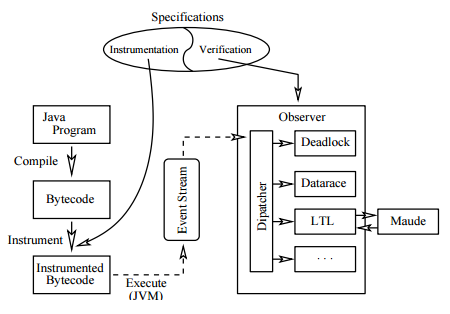
\includegraphics[width=100mm]{jpax.png}
\caption{JPaX Architecture (from \cite{havelund2001java})}
\label{img:jpax}
\end{center}
\end{figure}

JavaMaC \citep{kim2004java} is a ``run-time assurance system'' for Java programs while Mac means Monitoring and Checking. Its architecture is shown in Figure \ref{img:javamac}. Two definition languages are proposed: one for high-level specification which specifies required properties, another for low-level specification which defines the events and conditions. During the preparation, a ``filter'' and an ``event recognizer'' which are used to collect the necessary event traces are generated from the low-level specification, and a ``run-time checker'' is generated from the high-level spec. When running with the target program, events collected by the ``filter'' and ``event recognizer'' are sent to the ``run-time'' checker which is then responsible for the runtime verification work.

\begin{figure}[h]
\begin{center}
\centering
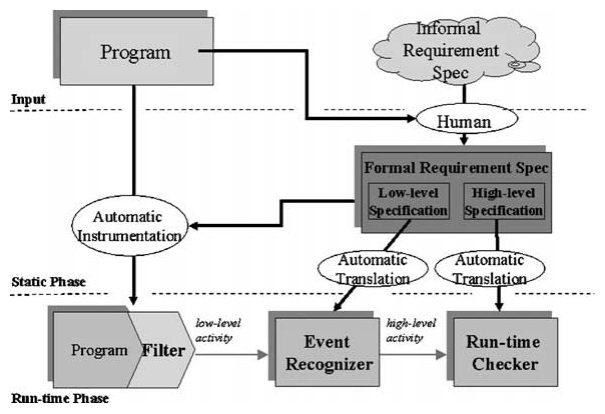
\includegraphics[width=100mm]{javamac.png}
\caption{MaC Architecture (from \cite{kim2004java})}
\label{img:javamac}
\end{center}
\end{figure}

\cite{d2005event} presents a logic named HAWK and its tools for RV of Java programs. HAWK is in fact built on EAGLE, another temporal logic which is considered more expressive \citep{barringer2004rule}. Although HAWK is event-based in contrast to state-based EAGLE, HAWK specifications are translated to EAGLE monitors. As Figure \ref{img:eagle} describes, during program execution, the EAGLE state is updated by instrumented program which then notifies the EAGLE observer. After that, the observer assesses the formul\ae{} in the current state to produce a result. 

\begin{figure}[h]
\begin{center}
\centering
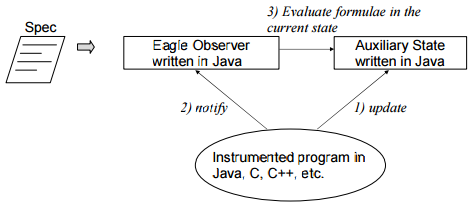
\includegraphics[width=100mm]{eagle.png}
\caption{Eagle Architecture (from \cite{d2005event})}
\label{img:eagle}
\end{center}
\end{figure}

Temporal Rover \citep{drusinsky2000temporal} is a commercial runtime verification tool based on LTL and MTL (Metric Temporal Logic). The specification code of Temporal Rover is inserted into the source code of Java, C, C++ or HDL and then converted into a compilable source file of corresponding language. A Temporal-Rover runtime verification system normally has two parts: host and target. The host is responsible for the verification while the target performs the computation of propositional formul\ae{} and sends back the results to the host via serial port, RPC or other customizable protocol.

Each of the frameworks discussed above hardwires a different specification formalism, which suggests that a general specification formalism serving all purposes does not exist. To be more expressive and generic, \cite{chen2007mop} introduced customizable and extensible ``logic-plugins'' in their runtime framework MOP and designed its architecture shown in Figure \ref{img:mop} with two layers: one is called ``language clients'' which support different programming languages, while another is ``logic repository'' which includes and manages various ``logic-plugins'' to support different specification formalisms, such as LTL, CFG (context-free grammar), FSM (finite state machine) and ERE (Extended regular expression).

\begin{figure}[h]
\begin{center}
\centering
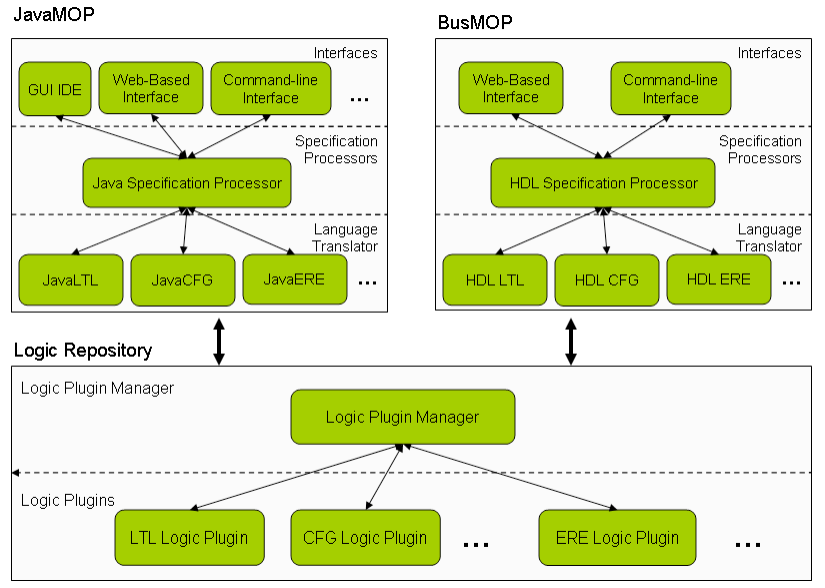
\includegraphics[width=130mm]{mop.png}
\caption{MOP Architecture (from \cite{chen2007mop})}
\label{img:mop}
\end{center}
\end{figure}
